\section{Exchange Heuristics}

In Combinatorial Optimization every solution $x$ is a subset of $B$.\\

An exchange heuristic \textbf{updates a current subset} $x^{(t)}$ step by step

\begin{enumerate}
	\item \textbf{Start} from a \textbf{feasible solution} $x^{(0)} \in X$ found somehow (often by a constructive heuristic).\\
	
	\item Generate a \textbf{family of feasible solutions} by exchanging elements, i.e. add subsets $A$ external to $x^{(t)}$ and delete subsets $D$ internal to $x^{(t)}$
	$$ x_{A,D}' = x \cup A \setminus D \text{ with } A \subseteq B \text{ and } D \subseteq x $$
	
	\item Use a \textbf{selection criteria} $\varphi (x, A, D)$ to choose the subsets to exchange
	$$ (A^\ast, D^\ast) = \arg \min_{(A,D)} \varphi (x, A, D) $$
	
	\item \textbf{Perform} the chosen \textbf{exchange} to generate the new current solution
	$$ x^{(t+1)} := x^{(t)} \cup A^\ast \setminus D^\ast $$
	
	\item If a \textbf{termination condition} holds, terminate; otherwise, go back to point 2
\end{enumerate}

\newpage

\subsection{Neighborhoods} 

An exchange heuristic is defined by:
\begin{enumerate}
	\item The \textbf{pairs of exchangeable subsets} $(A, D)$ in every solution $x$, i.e. the solutions generated by a single exchange starting from $x$.\\
	
	\item The \textbf{selection criteria} $\varphi (x, A, D)$.\\
\end{enumerate}

\textbf{Neighborhood} $N : \, X \rightarrow 2^X$ is a function which \textbf{associates to each feasible solution} $x \in X$ a \textbf{subset of feasible solutions} $N (x) \subseteq X$.\\

The situation can be formally \textbf{described with a search graph} in which
\begin{itemize}
	\item The \textbf{nodes} represent the \textbf{feasible solutions} $x \in X$.\\
	
	\item The \textbf{arcs connect each solution} $x$ \textbf{to those of its neighborhood} $N (x)$, moving elements into and out of $x$ (they are often denoted as moves).\\
\end{itemize}

Every run of the algorithm corresponds to a path in its search graph.\\

How does one define a neighborhood and select a move? \\

Essentially, it's the set of neighbor solutions, the one obtainable by one move, i.e. one set of exchanges.\\

\newpage

\subsubsection{Neighborhoods based on distance}

Every solution $x \in X$ can be represented by its \textbf{incidence vector}
$$ x_i = \begin{cases}
	1 & \text{ if } i \in x \\
	0 & \text{ if } i \in B \setminus x
\end{cases}$$
Associates 1 if the element is in the solution, 0 if it isn't; basically says which elements are in the solution and which ones aren't.\\

\textbf{Hamming distance} between two solutions $x$ and $x'$  is the \textbf{number of elements in which their incidence vectors differ}
$$ d_H (x, x') = \sum_{i \in B} |x_i - x_i'|$$
It adds, for each element $i \in B$, 1 if the element is in only one of the solutions and 0 if the element is in both/none of the solutions (fancy math way to count the differences).\\

Referring to the subsets, $d_H (x, x') = |x \setminus x'| + |x' \setminus x|$; equivalent definition, this is the cardinality of the elements that belong to one solution but not to the other.\\

A typical definition of neighborhood, with an integer parameter $k$, is the \textbf{set of all solutions with a Hamming distance from} $x$ \textbf{not larger than} $k$
$$ N_{H_k} (x) = \left\{x' \in X: \, d_H (x, x') \leq k \right\} $$

\newpage

\paragraph{Example:} The KP instance with $B = \{1, 2, 3, 4\}$, $v = [ \; 5 \; 4 \; 3 \; 2 \; ]$ and $V = 10$, has $13$ feasible solutions out of $16$ subsets

\begin{center}
	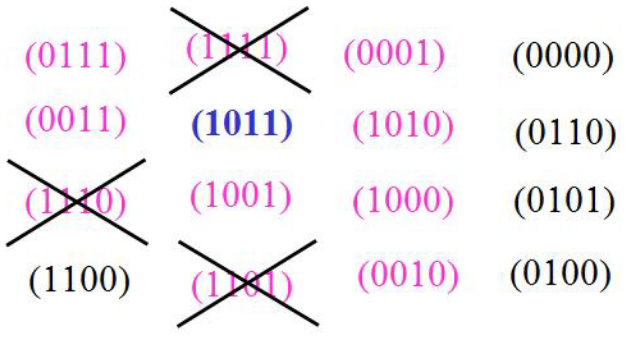
\includegraphics[width=0.6\columnwidth]{img/KPN1}
\end{center}

since subsets $\{1, 2, 3, 4\}, \{1, 2, 3\}$ and $\{1, 2, 4\}$ are unfeasible.\\

$10$ subsets (pink) have Hamming distance $\leq 2$ from $x = \{1, 3, 4\}$ (blue).\\

The neighborhood $N_{H_2} (x)$ consists of the $7$ feasible subsets in pink.\\
$N_{H_2} (x)$ excludes
\begin{itemize}
	\item the $3$ crossed subsets in pink because they are unfeasible
	
	\item the $5$ subsets in black because their Hamming distance from $x$ is $> 2$
\end{itemize}

The neighborhood must include only feasible solutions which respect the Hamming distance.\\

\newpage

\subsubsection{Neighborhoods based on operations}

Another common definition of neighborhood is obtained defining
\begin{itemize}
	\item a \textbf{family} $\mathcal{O}$ \textbf{of operations} on the solutions of the problem
	
	\item the \textbf{set of all solutions generated applying to} $x$ \textbf{the operations of} $\mathcal{O}$
	$$ N_{\mathcal{O}} (x) = \left\{x' \in X : \, \exists o \in \mathcal{O}: \, o (x) = x' \right\} $$
\end{itemize}

Considering again the KP, $\mathcal{O}$ can be defined as
\begin{itemize}
	\item \textbf{adding} to $x$ an element of $B \setminus x$
	
	\item \textbf{deleting} from $x$ at most an element (just to impose $x \in N (x)$)
	
	\item \textbf{swapping} one element of $x$ with one of $B \setminus x$
\end{itemize}

The resulting neighborhood $N_{\mathcal{O}}$ is related to those defined by the Hamming distance, but does not coincide with any of them
$$ N_{H_1} \subset N_{\mathcal{O}} \subset N_{H_2} $$
The Hamming distance 1 is just one operation, with this definition we can do more stuff, so it's bigger.\\

As the distance-based ones, these \textbf{neighborhoods can be parameterized} considering \textbf{sequences of} $k$ \textbf{operations} of $\mathcal{O}$ instead of a single one
$$ N_{\mathcal{O}_k} (x) = \left\{ x' \in X : \, \exists o_1, \, ... \, , o_k \in \mathcal{O} : \, o_k (o_{k-1} ( \, ... \, o_1 (x))) = x' \right\} $$ 
(bunch of operations, one after the other).\\

Essentially, define what you can do on a set (operations), and set a "number of operations away" distance metric.\\	

\newpage

\subsubsection{Distance and operation-based}

In general, an \textbf{operation-based} neighborhood includes solutions with \textbf{different Hamming distances from} $x$.\\

For the TSP one can define a neighborhood $N_{\mathcal{S}_1}$ including the solutions obtained swapping two nodes in their visit order

\begin{center}
	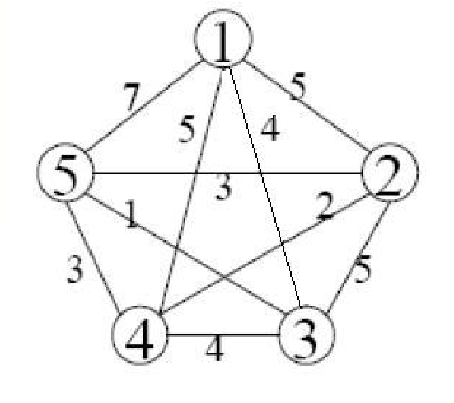
\includegraphics[width=0.5\columnwidth]{img/TSP2}
\end{center}

The neighborhood of solution $x = (3, 1, 4, 5, 2)$ is ($5$ vertices so $(5 \cdot 4) / 2$ pairs):
$$ \begin{array}{c c}
	N_{\mathcal{S}_1} (x) = & \{({\color{red} 1}, {\color{red} 3}, 4, 5, 2) , ({\color{red} 4}, 1, {\color{red} 3}, 5, 2) , ({\color{red} 5}, 1, 4, {\color{red} 3}, 2) , ({\color{red} 2}, 1, 4, 5, {\color{red} 3}) , (3, {\color{red} 4}, {\color{red} 1}, 5, 2) , \\
	& (3, {\color{red} 5}, 4, {\color{red} 1}, 2) , (3, {\color{red} 2}, 4, 5, {\color{red} 1}) , (3, 1, {\color{red} 5}, {\color{red} 4}, 2) , (3, 1, {\color{red} 2}, 5, {\color{red} 4}) , (3, 1, 4, {\color{red} 2}, {\color{red} 5}) \}
\end{array} $$
If the two nodes are adjacent, the modified arcs are $3 + 3$; otherwise, they are $4 + 4$.\\

This neighborhood cannot be defined as one with Hamming distance, in this case for this solution you include $4$ arcs less and $4$ more (to make the swap), $3$ if the node were adjacent, so the Hamming distance between two of these solutions would be $8$, $6$ in the case of adjacent nodes.\\
We can see that this neighborhood doesn't coincide with $N_{H_8}$ nor with $N_{H_6}$.\\

\newpage

\paragraph{Relations:} Sometimes the two definitions yield the same neighborhood
\begin{itemize}
	\item for the MDP
	\begin{itemize}
		\item $N_{H_2}$ (solutions at Hamming distance equal to $2$)
		\item $N_{\mathcal{S}_1}$ (swap one element of $x$ with one of $B \setminus x$)
	\end{itemize}
	\nn
	
	\item for the BPP
	\begin{itemize}
		\item $N_{H_2}$ (solutions at Hamming distance equal to $2$)
		\item $N_{\mathcal{T}_1}$ (transfer an object into a different container)
	\end{itemize}
	\nn
	
	\item for Max-SAT
	\begin{itemize}
		\item $N_{H_2}$ (solutions at Hamming distance equal to $2$)
		\item $N_{\mathcal{F}_1}$ ("flip" a variable: invert its truth assignment)
	\end{itemize}
	\nn
\end{itemize}

This is typical of problems with \textbf{solutions of fixed cardinality}:
\begin{itemize}
	\item perform a \textbf{sequence of} $k$ swaps between single elements $(|A| = |D| = 1)$: $k$ elements go into $x$ and $k$ elements go out
	
	\nn
	
	\item the \textbf{Hamming distance} between the two extreme solutions \textbf{is} $\leq 2k$ (if all exchanged elements are different, it is exactly $2k$)
\end{itemize}

\newpage

\paragraph{Different neighborhoods for the same problem:} the CMST.\\

Different ground sets yield different neighborhoods. In the CMST it is possible to set $B = E$ or $B = V \times T$
\begin{itemize}
	\item exchange \textbf{edges}: delete $(b, c)$, add $(b, e)$
	\begin{center}
		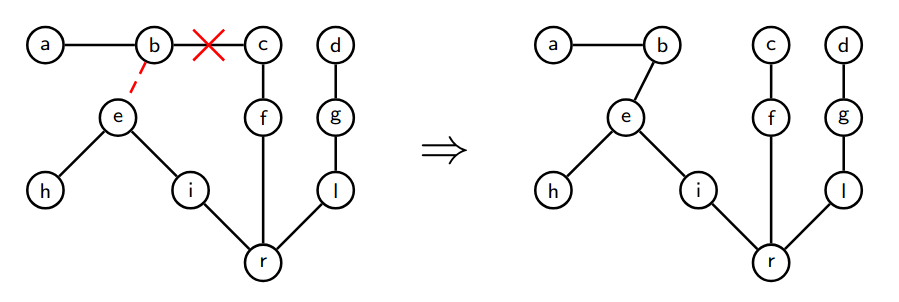
\includegraphics[width=0.85\columnwidth]{img/CMST1}
	\end{center}
	\nn
	
	\item exchange \textbf{vertices}: move $e$ from subtree 2 to subtree 1, and recompute the two minimum spanning subtrees
	\begin{center}
		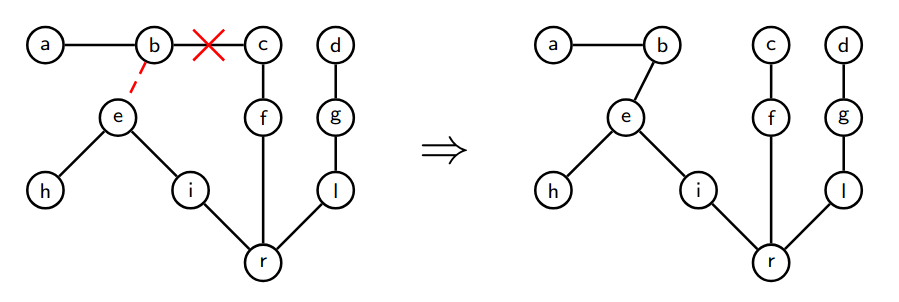
\includegraphics[width=0.85\columnwidth]{img/CMST1}
	\end{center}
\end{itemize}

\newpage

\textbf{PSMP:} For the PMSP it is possible to define
\begin{itemize}
	\item the transfer neighborhood $N_{\mathcal{T}_1}$, based on the set $\mathcal{T}_1$ of \textbf{all transfers} of a task on another machine
	\begin{center}
		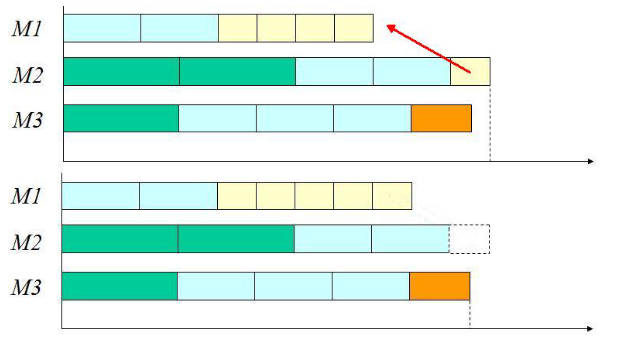
\includegraphics[width=0.7\columnwidth]{img/PSMP1}
	\end{center}
	\nn
	
	\item the swap neighborhood $N_{\mathcal{S}_1}$, based on the set $\mathcal{S}_1$ of the \textbf{swaps of two tasks} between two machines (one task for each machine)
	\begin{center}
		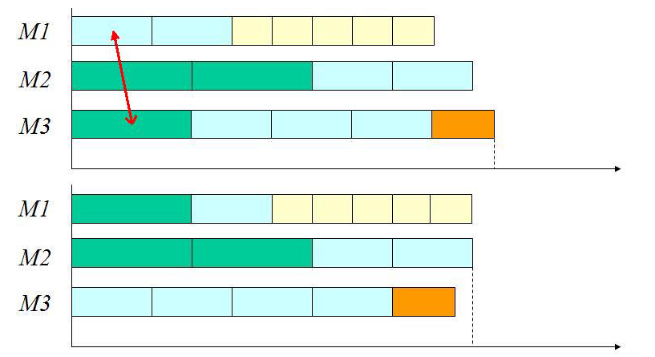
\includegraphics[width=0.7\columnwidth]{img/PSMP2}
	\end{center}
	\nn
\end{itemize}

\newpage

\subsubsection{Connectivity of the search graph}

An exchange heuristic can return the optimum only if \textbf{every feasible solution} can \textbf{reach} at least \textbf{one optimal solution}, that is there is a path from $x$ to $X^\ast$ for every $x \in X$.\\

Such a search graph is denoted as \textbf{weakly connected} to the optimum.\\

Since $X^\ast$ is unknown, a \textbf{stronger condition} is often used: a search graph is \textbf{strongly connected} when it admits a path from $x$ to $y$ for every $x, y \in X$.\\

A \textbf{good neighborhood} should guarantee some \textbf{connectivity conditions}
\begin{itemize}
	\item in the MDP, neighborhood $N_{\mathcal{S}_k}$ connects any pair of solutions with at most $k$ swaps
	
	\item in the KP and the SCP, no neighborhood $N_{\mathcal{S}_k}$ gives that guarantee (feasible solutions can have any cardinality)
	
	\item the search graph becomes connected also in the KP and the SCP if swaps are combined with both additions and deletions
\end{itemize}

Strong connectivity is when every feasible solution is reachable from every other feasible solution. Everything is connected.\\

If feasibility is defined in a sophisticated way, exchanging, adding and deleting \textbf{single} elements can be \textbf{insufficient} to reach all solutions: the \textbf{unfeasible subsets} can \textbf{break} all \textbf{paths} between some feasible solutions.

\begin{center}
	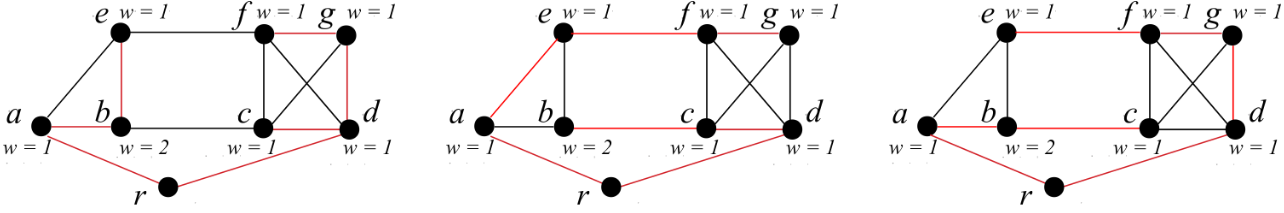
\includegraphics[width=\columnwidth]{img/connectivity}
\end{center}

If $V = 4$, only three solutions are feasible, all with two subtrees:
$$
\begin{array}{c c}
	x & = \{(r , a) , (a, b) , (b, e) , (r , d) , (c, d) , (d, g ) , (f , g )\} \\
	x' & = \{(r , a) , (a, e) , (e, f ) , (r , d) , (c, d) , (b, c) , (f , g )\} \\
	x'' & = \{(r , a) , (a, b) , (e, f ) , (r , d) , (b, c) , (d, g ) , (f , g )\}
\end{array}
$$
The three solutions are mutually reachable only exchanging at least two edges at at time; exchanging only one yields unfeasible subsets.

\newpage

\subsection{Steepest descent (hill-climbing) heuristics}
Abandoning the concept of neighborhood, let's consider how to move within them, what is the selection criteria?\\

The \textbf{simplest selection criteria} $\varphi (x, A, D)$ is the \textbf{objective function} (it is used in nearly all exchange heuristics).\\

\textbf{When} $\varphi (x, A, D) = f (x \cup A \setminus D)$, the \textbf{heuristic moves from} $x^{(t)}$ \textbf{to} the best solution in $N (x^{(t)})$ (this is considering only the update in value, not recalculating the whole objective function, if it makes the computation easier).\\

To avoid cyclic behavior, \textbf{only strictly improving solutions} are accepted. You can't "go back", otherwise you risk visiting multiple times the same solutions (if an earlier solution was better why not going back to it?).\\
Consequently, \textbf{the best known solution is the last visited one}.\\

\textit{Steepest Descent} for minimization, \textit{Ascent/Hill-climbing} for maximization.
\begin{algorithm}
	\caption{Algorithm $SteepestDescent(I , x^{(0)})$}
	\begin{algorithmic}
		\STATE $x := x^{(0)}$
		\STATE Stop$ := false$
		\WHILE{Stop$=false$}
		\STATE $\overline{x} := \arg \min_{x' \in N(x)} f(x')$
		\IF{$f(\overline{x}) \geq f(x)$}
		\STATE Stop$ := true$
		\ELSE 
		\STATE $x := \overline{x}$
		\ENDIF
		\ENDWHILE
		\RETURN $(x, f (x))$
	\end{algorithmic}
\end{algorithm}
Note that the best solution is not saved, since it's always the last one.\\

\newpage

\subsubsection{Local and global optimality}
A steepest descent heuristic \textbf{terminates}, by definition, when it finds a \textbf{locally optimal solution}, that is a solution $\overline{x} \in X$ such that
$$ f (\overline{x}) \leq f (x) \text{ for each } x \in N (x) $$
A local optimum is the best (\textit{technically} not worse) solution inside a neighborhood. 

\begin{center}
	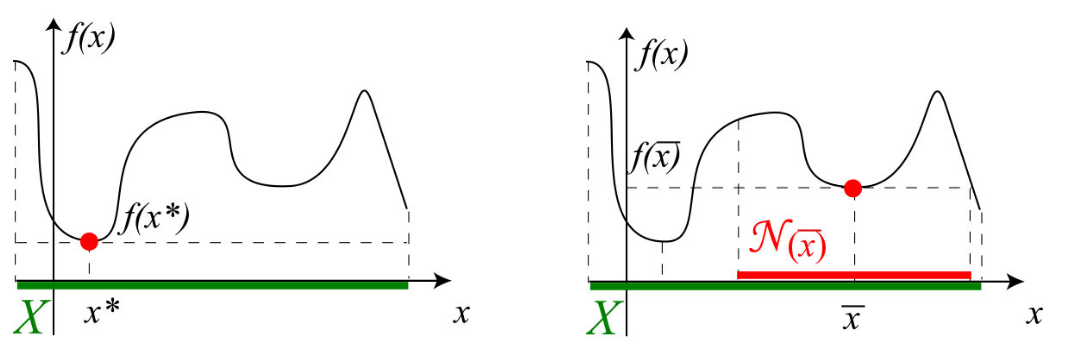
\includegraphics[width=\columnwidth]{img/localOptimum}
\end{center}

A globally optimal solution is always also locally optimal, but the opposite is not true in general: $X^\ast \subseteq \overline{X}_N \subseteq X$.\\

There could be a better solution outside the neighborhood, so the set of locally optimal solution is dependent on the definition of neighborhood.\\

\newpage

\subsubsection{Exact neighborhood}

\textbf{Exact neighborhood} is a neighborhood function $N : \, X \rightarrow 2^X$ such that \textbf{each local optimum is also a global optimum}
$$ \overline{X}_N = X^\ast $$

\textbf{Trivial case:} the neighborhood of each solution coincides with the whole feasible region ($N (x) = X$ for each $x \in X$, if I have the whole set I'm going to get the optimum). It's a useless neighborhood: too wide to explore.\\

The exact neighborhoods are \textbf{extremely rare}; examples: 
\begin{itemize}
	\item exchange between edges for the Minimum Spanning Tree problem
	
	\item exchange between basic and nonbasic variables used by the simplex algorithm for Linear Programming
\end{itemize}

In general, the steepest descent heuristic does not find a global optimum.\\

Its effectiveness depends on the properties of search graph and objective.\\

Essentially is a neighborhood that includes the global optimum; in general it's hard to obtain.\\

\newpage

\subsubsection{Properties of the search graph}
The properties of the graph can determine if our algorithm will find a "good" local optimum or a "bad" local optimum.\\

Some relevant properties for the effectiveness of an algorithm are
\begin{itemize}
	\item The \textbf{size of the search space} $|X|$ (big space needs big time, small space needs small time).\\
	
	\item The \textbf{connectivity of the search graph} (as discussed above, maybe the optimal solution is in a not connected part of the graph).\\
	
	\item The \textbf{diameter of the search graph}, that is the number of arcs of the minimum path between the two farthest solutions: larger neighborhoods produce graphs of smaller diameter (but other factors exist: see the "smallworld" effect).\\
\end{itemize}
\nn

Consider neighborhood $N_{\mathcal{S}_1}$ for the symmetric TSP on complete graphs
\begin{itemize}
	\item the search space includes $|X| = (n − 1)!$ solutions
	
	\item $N_{\mathcal{S}_1}$ (swap of two nodes) includes $\left(\begin{array}{c}
		n \\ 2 \end{array}\right) = n(n-1)/2$ solutions
	
	\item the search graph is strongly connected and has diameter $\leq n - 2$: every solution turns into another after at most $n - 2$ swaps.\\
	For example, $x = (1, 5, 4, 2, 3)$ becomes $x' = (1, 2, 3, 4, 5)$ in $3$ steps
	$$ x = (1, 5, 4, 2, 3) \rightarrow (1, 2, 4, 5, 3) \rightarrow (1, 2, 3, 5, 4) \rightarrow (1, 2, 3, 4, 5) = x' $$
	(the first node is always $1$, the last one is automatically in place)
\end{itemize}

\newpage

Other \textbf{relevant properties}:
\begin{itemize}
	\item The \textbf{density of global optima} $( |X^\ast|/|X |)$ \textbf{and local optima} $( | \overline{X}_N | / |X | )$: if the local optima are numerous, it is hard to find the global ones. \\
	How many global and local optima you have versus the total number of solutions. \\
	
	\item The \textbf{distribution of the quality} $\delta (\overline{x})$ \textbf{of local optima} (SQD diagram): if local optima are good, it is less important to find a global one. \\
	
	\item The \textbf{distribution of the locally optimal solutions in the search space}: if local optima are close to each other, it is not necessary to explore the whole space.\\
\end{itemize}

These indices would require an exhaustive exploration of the search graph.\\

In pratice, one performs a sampling and these analyses
\begin{itemize}
	\item require very long times
	\item can be misleading, especially if the global optima are unknown
\end{itemize}

\newpage

\paragraph{Example:} the TSP. For the TSP on a complete symmetric graph with Euclidean costs
\begin{itemize}
	\item The Hamming distance between two local optima is on average $\ll n$: the local optima concentrate in a small region of $X$.\\
	
	\item The Hamming distance between local optima on average exceeds that between local and global optima: the global optima tend to concentrate in the middle of local optima.\\
	
	\item The \textit{FDC} diagram (Fitness-Distance Correlation) reports the quality $\delta (\overline{x})$ versus the distance from global optima $d_H (\overline{x}, X^\ast)$ (for each local optima, on the horizontal axis is shown how far they are from the global, on the vertical axis there's the percentage deviation $\delta$): if they are correlated, better local optima are closer to the global ones.\\
\end{itemize}
\begin{center}
	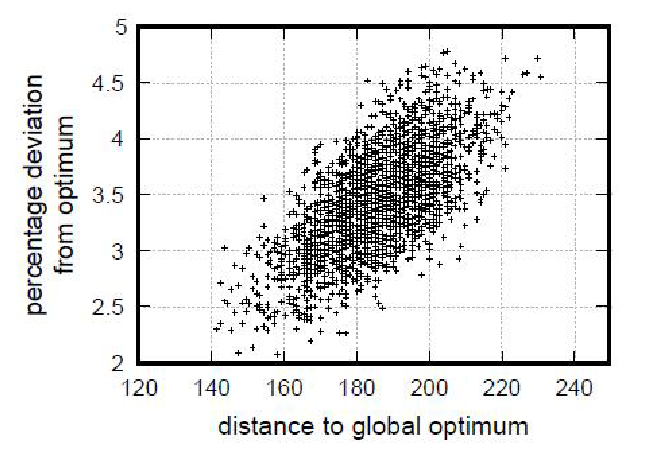
\includegraphics[width=0.7\columnwidth]{img/TSP3}
\end{center}

This diagram teaches that if, after you found a local optimum, it's good to (somehow) continue and intensify the search because you will probably move towards the global optimum.\\

\newpage

For the Quadratic Assignment Problem (QAP), the situation is different
\begin{center}
	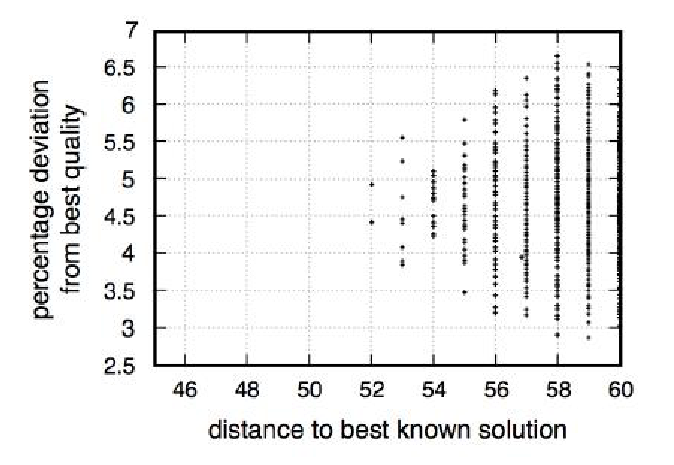
\includegraphics[width=0.7\columnwidth]{img/QAP}
\end{center}

If \textbf{quality} and \textbf{closeness} to the global optima are \textbf{strongly correlated}
\begin{itemize}
	\item It is \textbf{profitable} to \textbf{build good starting solutions}, because they drive the search near a good local optimum.\\
	
	\item It is \textbf{better} to \textbf{intensify} than to diversify.\\
\end{itemize}

If the \textbf{correlation is weak}
\begin{itemize}
	\item A good \textbf{initialization is less important}.\\
	
	\item It is \textbf{better} to \textbf{diversify} than to intensify
\end{itemize}

\newpage

\subsection{Landscape}
The \textbf{landscape} is the \textbf{triplet} $(X , N, f )$, where
\begin{itemize}
	\item $X$ is the \textbf{search space}, or the set of feasible solutions
	
	\item $N : X \rightarrow 2^X$ is the \textbf{neighborhood function}
	
	\item $f : X \rightarrow \mathbb{N}$ is the \textbf{objective function}
\end{itemize}

It is the \textbf{search graph with node weights given by the objective}. The first two terms correspond to the search graph, the last one gives weights to the nodes.\\

The \textbf{effectiveness} of steepest descent \textbf{depends} on the \textbf{landscape}
\begin{itemize}
	\item \textbf{smooth landscapes} yield few local optima, possibly of good quality, hence to \textbf{good results}
	
	\item \textbf{rugged landscapes} yield several local optima of widespread quality, hence to \textbf{bad results}
\end{itemize}

There is a \textbf{great variety of landscapes}, very different from one another
\begin{center}
	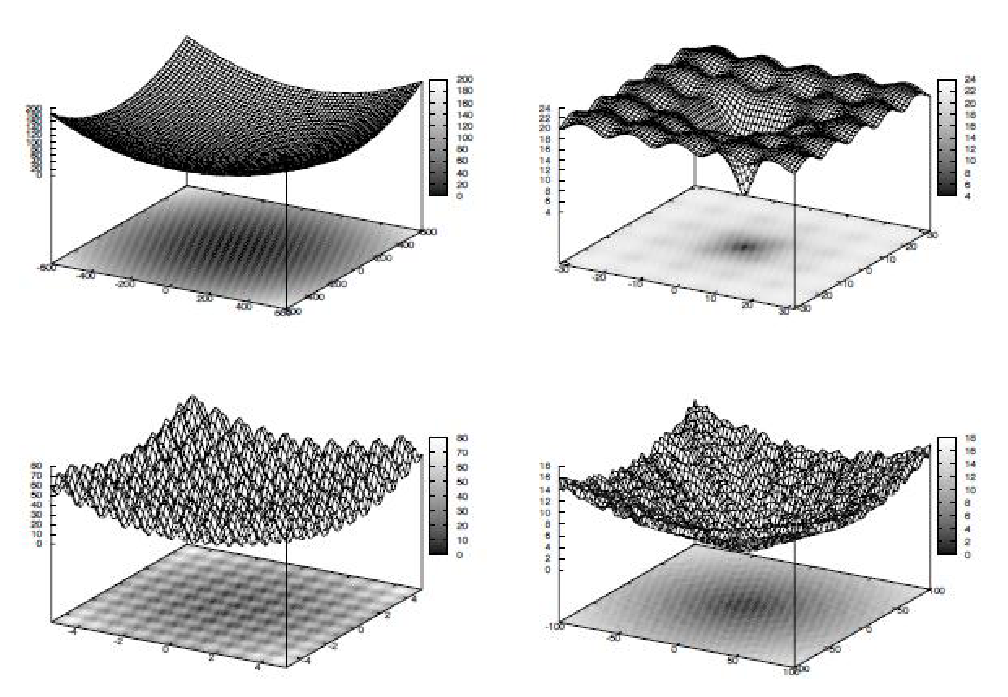
\includegraphics[width=0.9\columnwidth]{img/landscape1}
\end{center}

\newpage

\subsubsection{Autocorrelation coefficient}
The \textbf{complexity of a landscape} can be \textbf{empirically estimated}
\begin{enumerate}
	\item performing a \textbf{random walk} in the \textbf{search graph}
	
	\item determining the \textbf{sequence} of \textbf{values} of the \textbf{objective} $f^{(1)}, \, ... \, , f^{(t_{max})}$
	
	\item computing the \textbf{sample mean} 
	$$ \overline{f} = \frac{\displaystyle \sum_{t=1}^{t_{max}} f^{(t)}}{\displaystyle t_{max}} $$
	
	\item computing the \textbf{empirical autocorrelation coefficient}
	$$ r(i) = \frac{\displaystyle \frac{\displaystyle \sum_{t=1}^{t_{max} - i} \left(f^{(t)} - \overline{f}\right) \left(f^{(t+i)} - \overline{f}\right) }{\displaystyle t_{max} - i } }{\displaystyle \frac{\displaystyle \sum_{t=1}^{t_{max}} \left(f^{(t)} - \overline{f}\right)^2 }{\displaystyle t_{max} }}$$
	This is trying to relate the values of the objective function to the mean, with the goal of understanding how much these values vary; the denominator is the mean square error; the numerator is trying to know the difference between a step and the next, that way it can describe if the landscape is a smooth curve or a really rugged one (both could differ the same from the mean)
\end{enumerate}
That \textbf{relates} the \textbf{difference of the objective values in the solutions visited} with the \textbf{distance between these solutions along the walk}.\\

This is trying to give a function to describe the "ruggedness" of a landscape.\\

\newpage

Idea is:
\begin{itemize}
	\item With $i=0 \rightarrow r (0) = 1$ (perfect correlation at $0$ distance); numerator and denominator are the same, increasing the $i$ is considering "how much is the value changing?".\\
	
	\item In general $r (i)$ \textbf{decreases} as the \textbf{distance} $i$ \textbf{increases}.\\
	
	\item \textbf{If} $r (i) \approx 1$ in a large range of distances, the \textbf{landscape is smooth}:
	\begin{itemize}
		\item the neighbor solutions have values close to the current one
		\item there are few local optima
		\item the steepest descent heuristic is effective
	\end{itemize}
	\nn
	
	\item \textbf{If} $r (i)$ \textbf{varies steeply}, the \textbf{landscape is rugged}:
	\begin{itemize}
		\item the neighbor solutions have values far from the current one
		\item there are many local optima
		\item the steepest descent heuristic is ineffective
	\end{itemize}
	\nn
\end{itemize}

\newpage

\subsubsection{Plateau}
The \textbf{search graph} can be \textbf{partitioned} according to the \textbf{objective value}
\begin{itemize}
	\item \textbf{plateau of value} $f$ is each subset of solutions of value $f$ that are adjacent in the search graph (a bunch of equal values together)
\end{itemize}
\begin{center}
	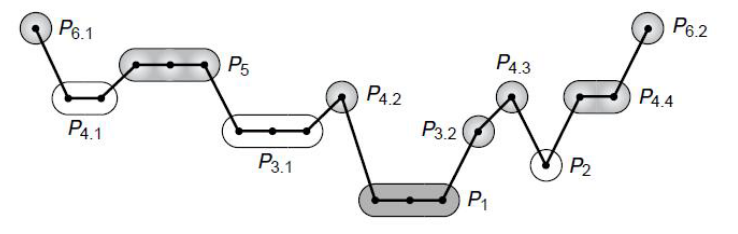
\includegraphics[width=0.7\columnwidth]{img/plateau1}
\end{center}

\textbf{Large plateaus complicate the choice of the solution}: most neighbors are equivalent, and the choice ends up depending on the visit order. An extremely uniform landscape is not an advantage.\\

Example: all transfers and swaps between machines 1 and 3 leave the objective value unchanged (most other moves worsen it)
\begin{center}
	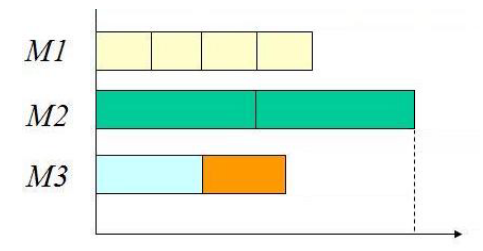
\includegraphics[width=0.55\columnwidth]{img/plateau2}
\end{center}

A plateau gives a lot of choices that are all effectively the same, making the objective function a bad criteria.\\

\newpage

\subsubsection{Attraction basins}
\textbf{Alternatively}, the \textbf{search graph} can be \textbf{partitioned} into:
\begin{itemize}
	\item \textbf{attraction basins} of the \textbf{locally optimal solutions} $\overline{x}$, that are the subsets of solutions $x^{(0)} \in X$ starting from which the steepest descent heuristic terminates in $\overline{x}$ (if I start with a steepest descent in the basin, I'm going to get $x$ since it's the closest local optimum)
\end{itemize}
\begin{center}
	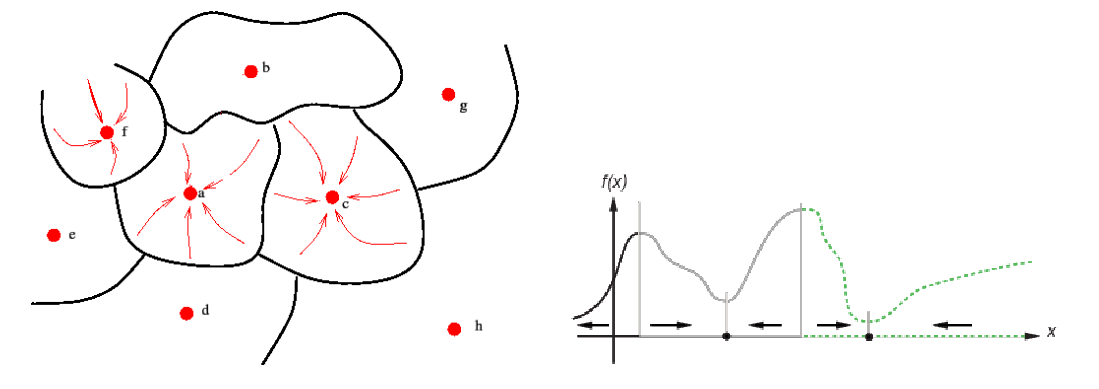
\includegraphics[width=\columnwidth]{img/basins}
\end{center}
The basins are separated by frontiers, on one side I get a local optimum, on the other side I get a different local optimum.\\ 

The steepest descent heuristic is
\begin{itemize}
	\item \textbf{Effective} if the attraction \textbf{basins} are \textbf{few and large} (especially if the global optima have larger basins), even if the algorithm will have to take a lot of steps.\\
	
	\item \textbf{Ineffective} if the attraction \textbf{basins} are \textbf{many and small} (especially if the global optima have smaller basins).\\
\end{itemize}

% End of L13

\newpage

\subsection{Complexity}
The complexity of the steepest descent heuristic depends on
\begin{itemize}
	\item The \textbf{number of iterations} $t_{max}$ \textbf{from} $x^{(0)}$ \textbf{to the local optimum found}, which depends on the structure of the search graph (width of the attraction basins) and is hard to estimate a priori.\\
	
	\item The \textbf{search for the best solution in the neighborhood} $(\overline{x})$, which depends on how the search itself is performed, but whose complexity estimation is usually standard.\\
\end{itemize}

\subsubsection{The exploration of the neighborhood}
It's the function in which you minimize the value of the objective.\\

\textbf{Two strategies} to explore the neighborhood are possible
\begin{enumerate}
	\item \textbf{Exhaustive search:} evaluate \textbf{all the neighbor solutions}; the complexity of a single step is the product of
	\begin{itemize}
		\item the number of neighbor solutions $(|N (x)|)$
		\item the evaluation of the cost of each solution $(\gamma_f (|B|, x))$
	\end{itemize}
	If it is not possible to generate only feasible solution:
	\begin{itemize}
		\item visit a superset of the neighborhood $( \tilde{N} (x) \supset N (x))$
		\item for each element $x$, evaluate the feasibility $(\gamma_X (|B|, x))$
		\item for the feasible ones, evaluate the cost $(\gamma_f (|B|, x))$
	\end{itemize}
	\nn
	
	\item \textbf{Efficient exploration} of the neighborhood \textbf{without a complete visit:} find the \textbf{best neighbor solution solving an auxiliary problem}. Only some special neighborhoods allow that.\\
\end{enumerate}

\newpage

\paragraph{Exhaustive visit of the neighborhood} \nn

\begin{algorithm}
	\caption{Algorithm $SteepestDescent(I , x^{(0)})$}
	\begin{algorithmic}
		\STATE $x := x^{(0)}$
		\STATE Stop $:= false$
		\WHILE{Stop $= false$}
		\STATE $ \tilde{x} := x$ // $\tilde{x} := \arg \min_{x' \in N(x)} f(x')$
		\FOR{each $x' \in \tilde{N}$}
		\IF{$x' \in N(x)$}
		\IF{$f(x') < f(\tilde{x})$}
		\STATE $\tilde{x} := x'$
		\ENDIF
		\ENDIF
		\ENDFOR
		\IF{$f(x') \geq f(x)$}
		\STATE Stop $ := true$
		\ELSE
		\STATE $x := \tilde{x}$
		\ENDIF
		\ENDWHILE
		\RETURN $(x, f (x))$
	\end{algorithmic}
\end{algorithm}

The \textbf{complexity} of the neighborhood exploration \textbf{combines} three terms
\begin{enumerate}
	\item $| \tilde{N} (x) |$: the \textbf{number of subsets visited}.\\
	
	\item $\gamma_X$: the \textbf{time to evaluate their feasibility}.\\
	
	\item $\gamma_f$: the \textbf{time to evaluate the objective} for a feasible solution.\\
\end{enumerate}

\newpage

\subsubsection{Evaluating or updating the objective}

\paragraph{The additive case:} The first way to accelerate an exchange algorithm is to \textbf{minimize the time to evaluate the objective}: in particular, it is \textbf{faster} to \textbf{update} $f (x)$ rather \textbf{than to recompute} it.\\

The \textbf{update of an additive objective} $f (x) = \sum_{j \in x} \phi_j$ requires to
\begin{itemize}
	\item Sum $\phi_i$ for each element $i \in A$, added to $x$.\\
	
	\item Subtract $\phi_j$ for each element $j \in D$, deleted from $x$
	$$ \delta f (x, A, D) = f (x \cup A \setminus D) - f(x) = \sum_{i \in A} \phi_i - \sum_{j \in D} \phi_j $$
	\nn
\end{itemize}

Examples: swap of objects (KP), columns (SCP), edges (CMSTP), ...\\

This \textbf{update} has \textbf{two} fundamental \textbf{properties}:
\begin{itemize}
	\item It takes \textbf{constant time for a constant number of elements} $|A| + |D|$.\\
	
	\item $\delta f (x, A, D)$ \textbf{does not depend on} $x$ (only on the elements added and deleted, more about it later).\\
\end{itemize}

If the objective function is additive just add and subtract the changes.\\

\newpage

\paragraph{The quadratic case:} The MDP has a quadratic objective function: computing it costs $\Theta (n^2)$.\\

Moving from $x$ to $x' = x \setminus \{i\} \cup \{j\}$ (neighborhood $N_{\mathcal{S}_1}$, just making a swap), the \textbf{update is}
$$ \delta f (x,i,j) = f \left(x \setminus \left\{i\right\} \cup \left\{j\right\}\right) - f(x) = \sum_{h,k \in x \setminus \left\{i\right\} \cup \left\{j\right\}} d_{hk} - \sum_{h,k \in x} d_{hk} $$

Which \textbf{depends on} $O (n)$ distance terms, related to points $i$ and $j$ (everything else cancels out).\\

There is a general trick \textbf{for the symmetric quadratic functions} with $d_{ii} = 0$

$$ \delta f (x,i,j) = \sum_{h \in x \setminus \left\{i\right\} \cup \left\{j\right\}} \; \sum_{k \in x \setminus \left\{i\right\} \cup \left\{j\right\}} d_{hk} - \sum_{h \in x} \; \sum_{k \in x} d_{hk} \implies $$
$$ \implies \delta f (x,i,j) = 2 \sum_{k \in x} d_{jk} - 2 \sum_{k \in x} d_{ik} - 2 d_{ij} = 2 \left(D_j (x) - D_i (x) - d_{ij}\right) $$

If $D_{\ell} (x) = \sum_{k \in x} d_{\ell k}$ is known for each $\ell \in B$, \textbf{the computation takes} $O (1)$.\\

If you save the distance from every element to the solution (distance from every other element in the solution set) there's no need to calculate $D_j (x)$ and $D_i (x)$ (distance from point $j$ and $i$ to the solution) every time, leaving out only $d_{ij}$, which has to be subtracted (since we don't have $i$ anymore) and can be done in constant time.\\

From the objective function we just need to add the distances relative to $j$ (represented in $D_j (x)$), subtract the distances from $i$ to the other elements in the solution ($D_i (x)$), and also subtract the distance from $j$ to $i$, since $i$ is not in the solution anymore. If we keep an auxiliary data structure for the distances $D_{\ell} (x)$ for every $\ell \in x$ then this update takes constant time. The auxiliary structures will have to be updated in $O (n)$ time each iteration. \\

\newpage


Example: the MDP
\begin{center}
	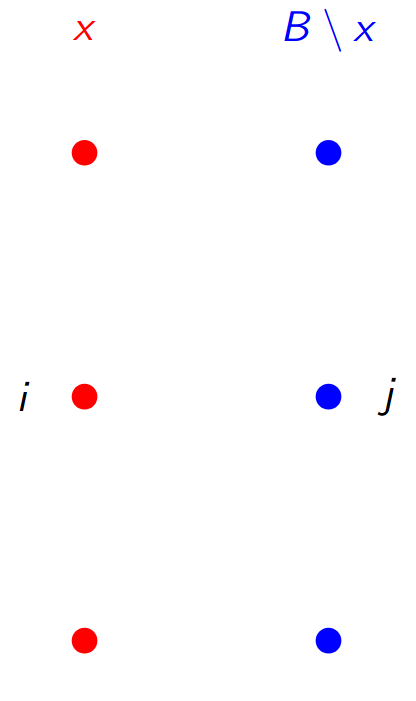
\includegraphics[width=0.25\columnwidth]{img/MDP2}
\end{center}
Let us consider $f (x) /2$.\\

Evaluate the exchange
$$ x \rightarrow x' = x \setminus \{i\} \cup \{j\} $$
with $i \in x$ and $j \in B \setminus x$ (swapping $i$ from the solution with $j$ from outside, $i$ becomes blue, $j$ becomes red).\\

$$ f (x') = f (x) − D_i + D_j − d_{ij} $$

\begin{itemize}
	\item the pairs including $i$ are lost
	\item the pairs including $j$ are acquired
	\item but the pair $(i, j)$ is in excess
\end{itemize}
The cost is computed in $O (1)$ time for each solution.\\

\textbf{Update of the data structures}:
$$ D_{\ell} = D_{\ell} - d_{\ll i} + d_{\ell j} \;\;\; \ell \in B $$
For each element $\ell \in B$
\begin{itemize}
	\item $d_{\ll i}$ disappears
	\item $d_{\ell j}$ appears
\end{itemize}

The auxiliary data structure is updated in $O (n)$ time for each iteration.\\

\newpage

\paragraph{Nonlinear examples:} Many nonlinear functions can be updated with similar tricks
\begin{itemize}
	\item save aggregated information on the current solution $x^{(t)}$
	
	\item use it to compute $f (x')$ efficiently for each $x' \in N (x^{(t)})$
	
	\item update it when moving to the following solution $x^{(t+1)}$
\end{itemize}

Using the transfer ($N_{\mathcal{T}_1}$) and swap ($N_{\mathcal{S}_1}$) neighborhoods for the PMSP, the objective can be updated in constant time by managing
\begin{enumerate}
	\item the completion time for each machine
	
	\item the indices of the machines with the first and second maximum time
\end{enumerate}

\begin{center}
	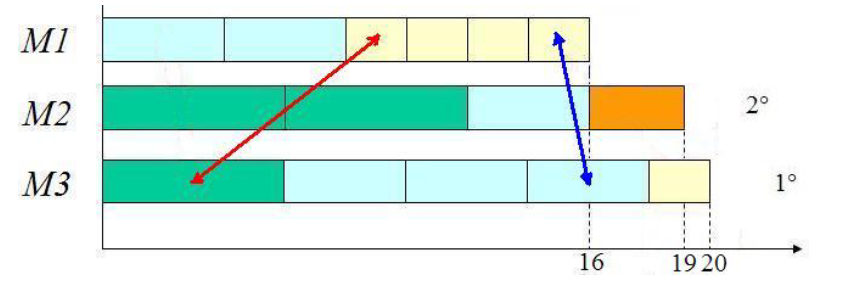
\includegraphics[width=0.75\columnwidth]{img/PMSP2}
\end{center}

Consider the swap $o = (i, j)$ of tasks $i$ and $j$ ($i$ on machine $M_i$, $j$ on machine $M_j$)
\begin{itemize}
	\item compute in constant time the new completion times: one increases, the other decreases (or both remain constant)
	
	\item test in constant time whether either exceeds the maximum
	
	\item if the maximum time decreases, test in constant time whether the other time or the second maximum time becomes the maximum
\end{itemize}

Once the neighborhood is visited and the exchange selected, update
\begin{itemize}
	\item the two modified completion times (each one in constant time)
	
	\item their positions in a max-heap (each one in time $O (\log |M|)$)
\end{itemize}
\nn	

Basically, compute the new the times, check if there's a new maximum, check if the maximum is still the maximum (if needed), then update the data structures. \\

To do this we need to remember: completion time for each machine and which machines have the maximum and the second maximum time.

\newpage

\paragraph{Use of local auxiliary information:} The auxiliary information used to compute $f (x')$ can be
\begin{itemize}
	\item \textbf{global}, that is referring to the \textbf{current solution} $x$
	
	\item \textbf{local}, that is referring to the \textbf{solution} $p_N (x')$ \textbf{visited before} $x'$ in neighborhood $N (x)$ according to a suitable order
\end{itemize}

Consider the neighborhood $N_{\mathcal{R}_2}$ for the asymmetric TSP:
\begin{itemize}
	\item the neighbor solutions differ from $x$ for $O (n)$ arcs
	
	\item general neighbor solutions differ from each other for $O (n)$ arcs
	
	\item if the pairs of arcs $(s_i , s_{i+1})$ and $(s_j , s_{j+1})$ follow the lexicographic order, the reverted path changes only by one arc
\end{itemize}

\begin{center}
	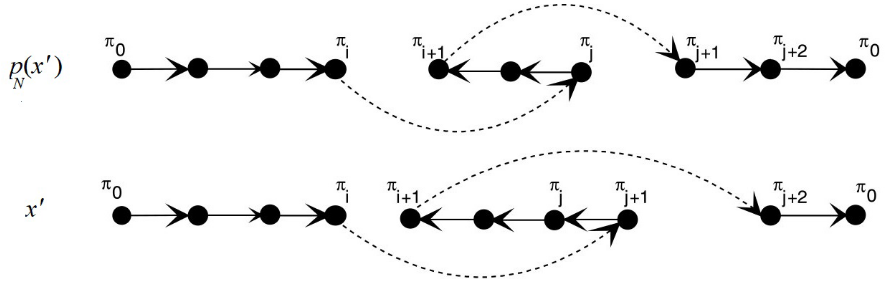
\includegraphics[width=0.9\columnwidth]{img/TSP4}
\end{center}

The \textbf{variation} of $f (x)$ between \textbf{two generic neighbor} solutions is
$$ \delta f (x, i, j) = c_{s_i ,s_j} + c_{s_{i+1}, s_{j+1}} - c_{s_i ,s_{i+1}} - c_{s_j ,s_{j+1}} + c_{s_j \, ... \, s_{i+1}} - c_{s_{i+1} \, ... \, s_j} $$

but moving from exchange $(s_i , s_j )$ to exchange $(s_i , s_{j+1})$
\begin{itemize}
	\item the first four terms change, but they can be checked in constant time
	
	\item the last two terms can be updated in constant time
	$$ \begin{cases}
		c_{s_{j'} \, ... \, s_{i+1}} & = c_{s_j \, ... \, s_{i+1}} + c_{s_{j+1},s_j} \\
		c_{s_{i+1} \, ... \, s_{j'}} & = c_{s_{i+1} \, ... \, s_j} + c_{s_j ,s_{j+1}}
	\end{cases}$$
\end{itemize}

Add the two arcs added (from $i$ to $j$ and from $i+1$ and $j+1$), remove the arcs that have been removed (from $i$ to $i+1$ and from $j$ to $j+1$), add the cost of the now reversed path, minus the cost of the original path. The last two terms (which can be big) can be updated in constant time by adding the new terms.\\
In constant time, with $6$ terms the function can be updated.\\

Is it acceptable to explore the neighborhood in a predefined order?

\newpage

\subsection{Feasibility of the neighborhood}
\textbf{Defining neighborhoods} with the Hamming distance or with operations \textbf{can generate} also \textbf{unfeasible subsets}, that \textbf{must be removed}

$$ \tilde{N}_{H_k} (x) = \{x' \subseteq B : \, d (x', x) \leq k \} \supseteq N_{H_k} (x) = \tilde{N}_{H_k} (x) \cap X $$

$$ \tilde{N}_{\mathcal{O}} (x) = \{ x' \subseteq B : \, \exists o \in \mathcal{O} : \, o (x) = x' \} \supseteq N_{\mathcal{O}} (x) = \tilde{N}_{\mathcal{O}} (x) \cap X $$

(Examples: KP, BPP, SCP, CMSTP, \dots).\\

If it is not possible to avoid a priori the unfeasible subsets, one must
\begin{itemize}
	\item \textbf{Test} the \textbf{feasibility of each element} of $\tilde{N} (x)$ to obtain $N (x)$.\\
	
	\item For the feasible elements, \textbf{evaluate} the \textbf{cost}.\\
\end{itemize}

The feasibility test can be made efficient with techniques similar to the ones used for the objective evaluation.\\

Example: update in constant time the total volume of a subset in the KP.\\

\newpage

\paragraph{Example:} The CMSTP. Consider the swap neighborhood $N_{\mathcal{S}_1}$ (add one edge, delete another)
\begin{itemize}
	\item If the two edges are in the same branch, the solution remains feasible.\\
	
	\item If they are in different branches, one loses weight, the other acquires it: the variation is equal to the weight of the subtree transferred.\\
\end{itemize}

\begin{center}
	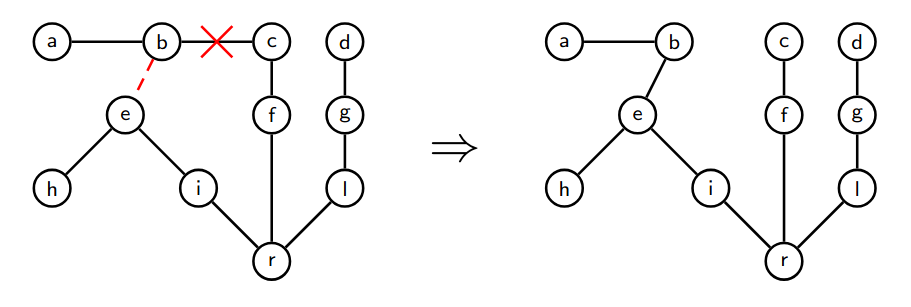
\includegraphics[width=0.8\columnwidth]{img/CMST3}
\end{center}

If each vertex saves the weight of its appended subtree, to test feasibility compare this weight with the residual capacity of the receiving branch (the weight appended to $b$ with the residual capacity of the left branch).\\

Once the best exchange is performed, the information must be updated in time $O (n)$ visiting the old ancestors from $c$ and the new ones from $e$.\\

If you know the total weight of the branch that has been cut (how many vertices are still appended) and confront that value with the residual capacity of the receiving branch.\\

You can save in a vector the total weight of the subtree appended to each vertex in the current solution. After a move you need to update all auxiliary information.\\

\newpage

\subsection{Partial saving of the neighborhood}

When performing an \textbf{operation} $o \in \mathcal{O}$ on a \textbf{solution} $x \in X$ sometimes
\begin{itemize}
	\item the \textbf{feasibility of the resulting solution} $o (x)$
	\item the \textbf{variation of the objective} $\delta f_o (x) = f (o(x)) − f (x)$
\end{itemize}
\textbf{depend only on a part of} $x$ (possibly, very small).\\

For example, consider the swap neighborhood $N_{\mathcal{S}_1}$ for the CMST:
\begin{itemize}
	\item add an edge $k \in B \setminus x$
	\item delete an edge $h \in x$
\end{itemize}
Two branches are involved: one acquires a subtree, the other loses it.\\

The \textbf{feasibility of swap} $(i, j)$ \textbf{depends} on the \textbf{branches including} $i$ \textbf{and} $j$: it is the \textbf{same in} $x$ \textbf{and} $x'$ and is \textbf{not affected by swap} $(h, k)$
$$ \delta f_{i,j} (x) = \delta f_{i,j} (x') $$

\textbf{For each operation} $o ∈ \tilde{\mathcal{O}} \subset \mathcal{O}$ \textbf{and for each} $x' = o (x)$
\begin{itemize}
	\item $o (x')$ is \textbf{feasible} if and only \textbf{if} $o (x)$ is \textbf{feasible}
	\item $\delta f_o (x') = \delta f_o (x)$
\end{itemize}

It is then \textbf{advantageous} to
\begin{enumerate}
	\item compute and \textbf{save} $\delta f_o (x)$ \textbf{for every} $o \in \mathcal{O}$, that is keep the set of feasible exchanges and their associated values $\delta f$
	
	\item \textbf{perform} the \textbf{best operation} $o^\ast$, and generate a new solution $x'$
	
	\item recompute and \textbf{save} $\delta f_o (x')$ \textbf{only for} $o ∈ \mathcal{O} \setminus \tilde{O}$, that is remove the exchanges on modified branches, recompute their values, and retrieve $\delta f_o (x')$ for all $o \in \tilde{\mathcal{O}}$ (their values are still correct)
	
	\item go back to point $2$
\end{enumerate}

If the branches are numerous, $|\mathcal{O} \setminus \tilde{\mathcal{O}}| \ll |\mathcal{O}|$ and the saving is very strong.\\
It is typical of problems whose solution is a partition.\\

TLDR: save the variance for small operations, it will be the same across solutions which differ from one another in parts not affected by such operation.\\

\newpage

\subsection{Trade-off between efficiency and effectiveness}
The \textbf{complexity} of an exchange heuristic \textbf{depends on three factors}
\begin{enumerate}
	\item \textbf{Number of iterations}.\\
	
	\item \textbf{Cardinality of the visited neighborhood}.\\
	
	\item \textbf{Computation of the feasibility and cost for the single neighbor}.\\
	
\end{enumerate}

The first two factors are clearly conflicting:
\begin{itemize}
	\item A \textbf{small neighborhood} is \textbf{fast to explore}, but requires \textbf{several steps} to \textbf{reach} a local \textbf{optimum}.\\
	
	\item A \textbf{large neighborhood} requires \textbf{few steps}, but is \textbf{slow to explore}.\\
\end{itemize}

The optimal \textbf{trade-off is somewhere in the middle}: a neighborhood
\begin{itemize}
	\item \textbf{large enough} to include \textbf{good solutions}
	\item \textbf{small enough} to be \textbf{explored quickly}
\end{itemize}

but it is hard to identify, because
\begin{itemize}
	\item \textbf{efficiency quickly worsens} as size increases
	\item the resulting \textbf{solution} also \textbf{changes with the neighborhood} (large ones have better local optima)
\end{itemize}

\newpage

It is also possible to \textbf{define a neighborhood} $N$ and \textbf{tune its size}, you can modify it
\begin{itemize}
	\item \textbf{Explore} only a \textbf{promising sub-neighborhood} $N′ ⊂ N$. For example, if the objective function is additive, one can
	\begin{itemize}
		\item add only elements $j \in B \setminus x$ of low cost $\phi_j$
		\item delete only elements $i \in x$ of high cost $\phi_i$
	\end{itemize}
	\nn
	
	\item \textbf{Terminate the visit after finding a promising solution}. For example, the first-best strategy stops the exploration at the first solution better than the current one
	\begin{center}
		If $f (\tilde{x}) < f (x)$ then $x := \tilde{x}$; Stop $:= true$;
	\end{center}
	\nn
\end{itemize}

The \textbf{effectiveness depends on the objective}
\begin{itemize}
	\item if the \textbf{cost of some elements influences very much the objective}, it is worth taking it into account, fixing of forbidding them
\end{itemize}

\textbf{and} on the \textbf{structure of the neighborhood}
\begin{itemize}
	\item if the \textbf{landscape is smooth}, the first improving solution approximates well the best solution of the neighborhood: it is better to stop
	
	\item if the \textbf{landscape is rugged}, the best solution of the neighborhood could be much better: it is better to go on
\end{itemize}

% End of L14

\newpage

\subsection{Very Large Scale Neighborhood Search}
\textbf{Larger neighborhoods} yield in general \textbf{larger attraction basins}, so that
\begin{itemize}
	\item the \textbf{steepest descent} heuristic becomes very \textbf{effective}
	\item but the \textbf{exploration time is longer}
\end{itemize}

The \textbf{Very Large Scale Neighborhood (VLSN)} Search approaches have
\begin{itemize}
	\item \textbf{neighborhoods exponential} in $|B|$ (or high-order polynomial)
	\item \textbf{explored} in low-order \textbf{polynomial time} (it's just another CO problem, finding the best solution in a finite set)
\end{itemize}

Two strategies allow limiting the computational time
\begin{enumerate}
	\item select a neighborhood in which the \textbf{objective can be optimized} without an exhaustive exploration
	\item \textbf{explore the neighborhood heuristically} and \textbf{return} a \textbf{promising neighbor solution}, instead of the best one
\end{enumerate}

\newpage

\subsubsection{Efficient visit of exponential neighborhoods}

Neighborhoods can be easily \textbf{parameterized}
$$ N_{\mathcal{O}_k} (x) = \left\{ x' \in X : x' = o_k (o_k−1 (\, ... \, o_1 (x))) \text{ with } o_1, \, ... \, , o_k \in \mathcal{O} \right\} $$

and it would be nice to \textbf{tune the number of operations} $k$
\begin{itemize}
	\item increasing $k$ when necessary to improve the current solution $x$
	
	\item decreasing $k$ when sufficient to improve the current solution $x$
\end{itemize}

The idea is to \textbf{define a composite move} as a \textbf{set of elementary moves} (that is a combinatorial optimization problem).\\

\textbf{Finding the optimal solution} in such neighborhoods \textbf{requires solving an auxiliary problem}, typically on a matrix or graph
\begin{itemize}
	\item \textbf{set packing:} Dynasearch
	
	\item \textbf{negative cost circuit:} cyclic exchanges
	
	\item \textbf{shortest path:} ejection chains, order-and-split
\end{itemize}

Such auxiliary tools are usually defined improvement matrices or graphs.\\

\paragraph{Combining elementary moves into composite ones:} An operation $o \in \mathcal{O}$ usually modifies only some components of solution $x$. Often \textbf{only the modified components of} $x$ \textbf{determine}
\begin{itemize}
	\item the \textbf{feasibility} of the \textbf{new subset} $o (x)$
	
	\item the \textbf{variation of the objective function} $\delta f_o (x) = f (o (x)) - f (x)$
\end{itemize}

Then, \textbf{two operations} $o, o' \in \mathcal{O}$ that \textbf{modify different components} of $x$ 
\begin{itemize}
	\item are \textbf{compatible and commutable}
	$$ o' (o (x)) = o (o' (x)) \in X $$
	
	\item have an \textbf{overall effect independent of the order of application} and easy to compute: for additive functions it is usually the sum
	$$ \delta f_{oo'} (x) = \delta f_{o'o} (x) = \delta f_o (x) + \delta f_{o'} (x) $$
\end{itemize}

The idea is to \textbf{perform a whole set of moves combining their effects}.\\

\newpage

\subsubsection{Dynasearch}

Let a \textbf{composite move} be a \textbf{set of elementary moves} with mutually independent effects on feasibility and the objective.\\

The situation can be modeled with an \textbf{improvement matrix} $A$ in which 
\begin{itemize}
	\item the \textbf{rows} represent the \textbf{components of the solution} (e.g., branches in the CMSTP, circuits in the VRP, circuit segments in the TSP)
	
	\item the \textbf{columns} represent the \textbf{elementary moves} $o \in \mathcal{O}$ and the \textbf{value of a column} equals the \textbf{objective improvement} $- \delta f_o (x)$
	
	\item $a_{io} = 1$ \textbf{when move} $o$ \textbf{affects component} $i$, $a_{io} = 0$ otherwise
\end{itemize}

Determine an \textbf{optimum packing of the columns}, that is a subset of nonconflicting columns of maximum value.\\

The Set Packing Problem is in general $\mathcal{NP}$-hard, but
\begin{itemize}
	\item on special matrices it is polynomial (as in the matrix from the TSP)
	
	\item if each move modifies at most two components
	\begin{itemize}
		\item the rows can be seen as vertices of a graph
		\item the columns can be seen as edges of a graph
		\item each packing of columns becomes a matching
	\end{itemize}
	and the maximum matching problem is polynomial
\end{itemize}

\newpage

\subsubsection{Cyclic exchanges}
Another set of exponential neighborhood that can be explored in polynomial time.\\

In many problems
\begin{itemize}
	\item A \textbf{feasible solution} is a \textbf{partition of objects into components} $S^{(\ell)}$, that is an assignment of objects to components $(i, S_i )$ (vertices or edges into branches for the CMSTP, nodes or arcs into circuits for the VRP, objects into containers in the BPP, etc.; the ground set is a Cartesian product of vertices and subtrees, objects and containers, ecc.; a single solution is a partition).\\
	
	\item The \textbf{feasibility} is \textbf{associated to the single components} (the feasibility can be checked against the single component, such as container, subtree, ecc.).\\
	
	\item The \textbf{objective function is additive with respect to the components}
	$$ f (x) = \sum_{\ell = 1}^{r} f \left(S^{(\ell)} \right)$$
\end{itemize}

In these problems, it is natural to define the \textbf{set of operations} $\mathcal{T}_k$ which includes the \textbf{transfers of} $k$ \textbf{elements from their component to another} and to derive from $\mathcal{T}_k$ the \textbf{neighborhood} $N_{\mathcal{T}_k}$
\begin{itemize}
	\item Often the feasibility constraints forbid the simple transfers ($N_{\mathcal{T}_1}$ is often unfeasible, if all containers are full I can't simply put an object into another container).\\
	
	\item But the number of multiple transfers quickly grows with $k$.\\
\end{itemize}
We want to \textbf{find} a \textbf{subset of} $N_{\mathcal{T}_k}$ \textbf{large}, but \textbf{efficient} to explore.\\

\newpage

\subsubsection{The improvement graph} 
Allows to \textbf{describe sequences of transfers}
\begin{itemize}
	\item A \textbf{node} $i$ corresponds to an \textbf{element} $i$ of the \textbf{current solution} $x$.\\
	
	\item An \textbf{arc} $(i, j)$ corresponds to
	\begin{itemize}
		\item the \textbf{transfer} of \textbf{element} $i$ from its current \textbf{component} $S_i$ to the current \textbf{component} $S_j$ of element $j$
		\item the \textbf{deletion} of \textbf{element} $j$ from \textbf{component} $S_j$
	\end{itemize}
	\nn
	
	\item The \textbf{cost of arc} $c_{ij}$ corresponds to the (positive or negative) \textbf{variation of the contribution of} $S_j$ to the objective
	$$ c_{ij} = f (S_j \cup \{i\} \setminus \{j\}) - f (S_j) $$
	with $c_{ij} = +\infty$ \textbf{if} it is \textbf{unfeasible} to replace $j$ with $i$ in $S_j$
\end{itemize}

A circuit in such a graph corresponds to a closed sequence of transfers.\\

If I put $i$ in place of $j$, $j$ has to go somewhere, for example in the place of $k$, and so on, until I have a feasible sequence of transfer, i.e. a cycle in the improvement graph (each move must belong to a different component, otherwise problems).\\

The \textbf{cost of the circuit} corresponds to the \textbf{cost of the sequence}
\begin{itemize}
	\item but only \textbf{if each node belongs to a different component}
\end{itemize}

Find the \textbf{minimum cost circuit} satisfying this condition.\\

\newpage

\paragraph{Example:} the CMSTP
\begin{center}
	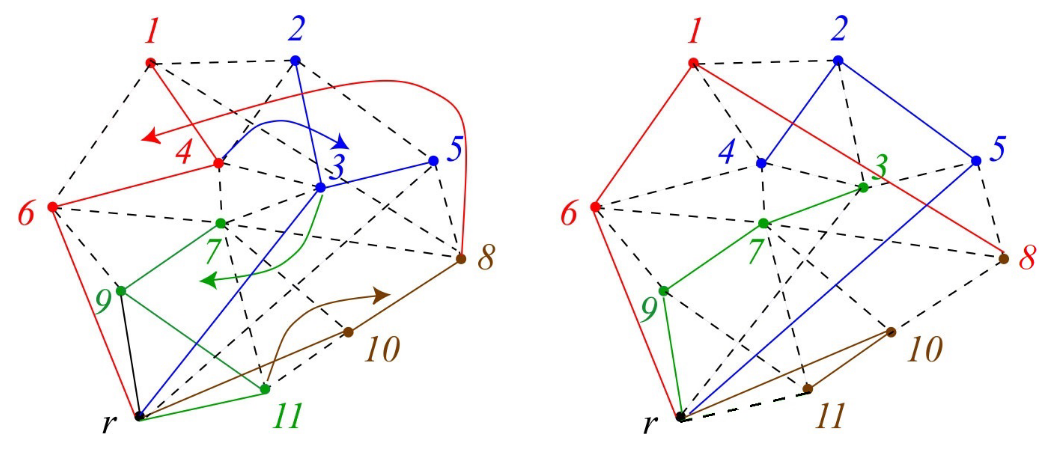
\includegraphics[width=0.9\columnwidth]{img/CMSTP1}
\end{center}
Consider the composite move $(4, {\color{blue} 3}), (3, {\color{green} 11}), (11, {\color{brown} 8}), (8, {\color{red} 4})$:
\begin{itemize}
	\item $4$ moves into the blue branch to replace $3$
	\item $3$ moves into the green branch to replace $11$
	\item $11$ moves into the brown branch to replace $8$
	\item $8$ moves into the red branch to replace $4$
\end{itemize}

The cost variation for subtree $S_j$ yields the cost of arc $c_{ij}$.\\

The weight of branch $S_j$ varies by $w_i - w_j$: if unfeasible, forbid the arc. The feasibility is determined by the single transfer, if the new cost is still feasible the transfer is feasible.\\

The total cost is the sum of all variation due to the transfers made.\\

If you visit two elements in a single component it is not guaranteed that the feasibility depends only on the single transfer.\\

\newpage

\paragraph{Search for the minimum cost circuit:} The problem is actually $\mathcal{NP}$-hard, but
\begin{itemize}
	\item The constraint of visiting only once each component allows a rather efficient \textbf{dynamic programming algorithm} that grows partial paths (if the components are $r$, the circuit has at most $r$ arcs).\\
	
	\item All \textbf{partial paths of cost} $\geq 0$ \textbf{can be neglected} because
	\begin{itemize}
		\item the total variation of the objective sums the effect of the single moves
		$$ \delta f_{o_1, \, ... \, , o_k} (x) = \sum_{\ell = 1}^k \delta f_{o_{\ell}} (x) $$
		
		\item every \textbf{sequence} of numbers \textbf{with negative sum} admits a cyclic permutation \textbf{whose partial sums are all negative}. e.g., $(+1, −2, +4, −10, +2)$ admits $(−10, +2, +1, −2, +4)$ (if the total is negative I can start with a big negative and stay in the negative all the way)
		
		\item therefore, \textbf{there is a cyclic permutation of the moves} $o_1, \, ... \, , o_k$
		$$ \delta f_{o_1, \, ... \, , o_k} (x) < 0 \implies \exists h : \, \delta f_{o_{(h+1) \mod k}, \, ... \, , o_{(h+\ell) \mod k}} (x) < 0 \text{ for } \ell = 1, \, ... \, , k $$
		that is, \textbf{improving at each step}.\\
	\end{itemize}
\end{itemize}

Moreover,
\begin{itemize}
	\item There are \textbf{heuristic polynomial algorithms} for the problem.\\
	
	\item There are \textbf{polynomial algorithms to solve relaxations} of the problem that neglect the constraint on the components, finding
	\begin{itemize}
		\item a nonminimum negative circuit (Floyd-Warshall), if any exists
		
		\item a circuit of minimum average cost (total cost divided by number of arcs)
	\end{itemize}
	If the cost of such relaxed solutions is
	\begin{itemize}
		\item positive, then no negative circuit exists
		
		\item negative, then the relaxed solution can be
		\begin{itemize}
			\item optimal (if luckily they are feasible)
			\item a starting point to generate a feasible heuristic solution
		\end{itemize}
	\end{itemize}
\end{itemize}

\newpage

\paragraph{Noncyclic exchange chains:} It is also possible to create noncyclic transfer chains, so that the cardinality of the components can vary.\\

It is enough to add to the improvement graph
\begin{itemize}
	\item A \textbf{source node} (fake, doesn't represent any node of the problem).\\
	
	\item A \textbf{node} for \textbf{each component} (a fake node for each component in the solution, for example each subtree).\\
	
	\item \textbf{Arcs} from the \textbf{source node} to the \textbf{nodes associated to the elements}.\\
	
	\item \textbf{Arcs} from the \textbf{nodes associated to the elements} to the \textbf{nodes associated to the components}.\\
\end{itemize}

Then, find the minimum cost path that
\begin{itemize}
	\item \textbf{starts} from the \textbf{source node}
	
	\item \textbf{ends} in a \textbf{component node}
	
	\item \textbf{visits at most one node for each component}
\end{itemize}

These paths correspond to \textbf{open transfer chains} in which
\begin{itemize}
	\item a component loses an element
	
	\item zero or more components lose an element and acquire another one
	
	\item a component acquires an element
\end{itemize}

You just get an element from a source node, swap $n$ elements among components, end in a component which does not lose an element.\\

\newpage

Example: the CMSTP
\begin{center}
	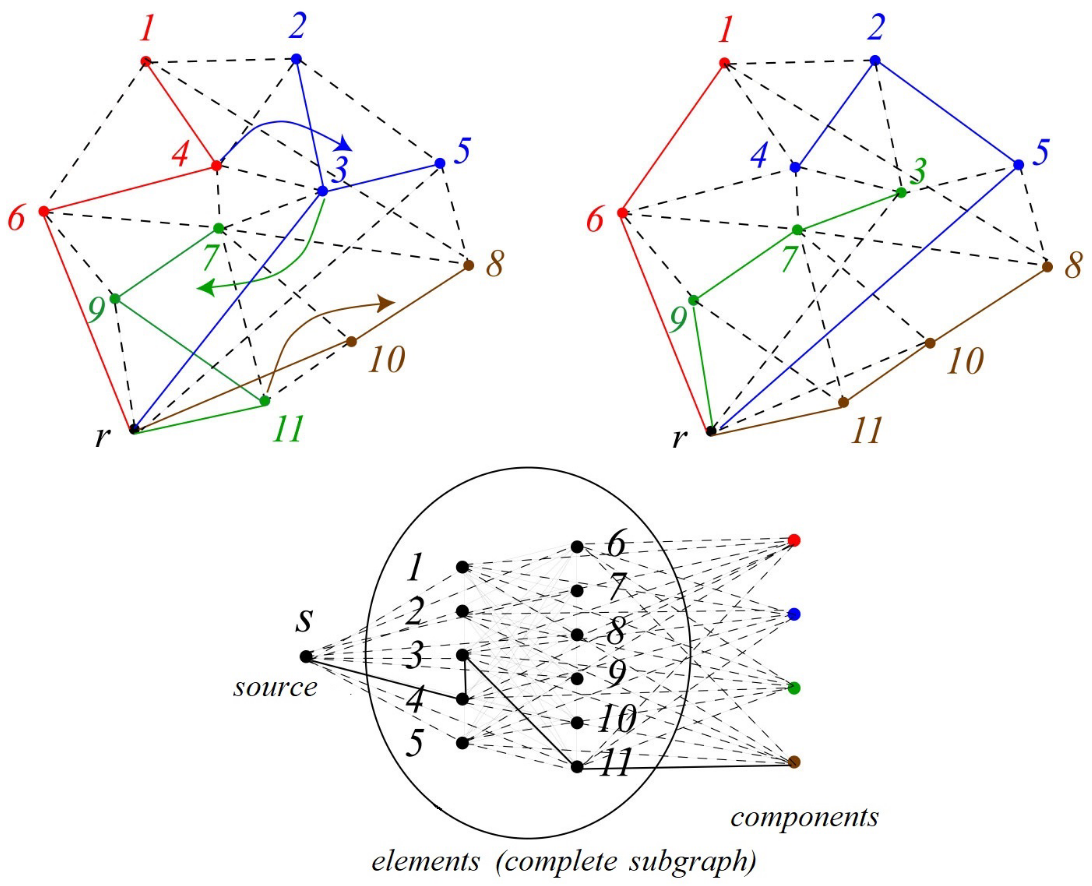
\includegraphics[width=0.9\columnwidth]{img/CMSTP2}
\end{center}
Noncyclic exchange $(s, {\color{red} 4}), (4, {\color{blue} 3}), (3, {\color{green} 11}), (11, {\color{brown} S_4})$.\\

4 goes to $s$ (it just means that we remove it), then we swap 4 and 3, and so on until in the green subtree we swap 11, which goes to brown, with $S_4$ (another fake element).\\

It's just a notation to denote empty first and last swaps.\\

\newpage

\subsection{Order-first split-second}

The \textbf{Order-first split-second} method for \textbf{partition problems}
\begin{itemize}
	\item \textbf{Builds} a \textbf{starting permutation of the elements} to be partitioned.\\
	
	\item \textbf{Partitions the elements into components in an optimum way} under the additional constraint that \textbf{elements} of the \textbf{same component} be \textbf{consecutive in the starting permutation}.\\
\end{itemize}

Of course, the solution depends on the starting permutation: it is reasonable to repeat the resolution for different permutations creating a two-level method
\begin{enumerate}
	\item the upper level selects a permutation
	
	\item the lower level computes the optimal partition for the permutation
\end{enumerate}

Problem: different permutations yield the same solution (the permutations are more numerous than the solutions).\\


\paragraph{The auxiliary graph:} Once again, we exploit an auxiliary graph. \\
Given the permutation $(s_1, \, ... \, , s_n)$ of the elements
\begin{itemize}
	\item each \textbf{node} $v_i$ \textbf{corresponds to an element} $s_i$ plus a fictitious node $v_0$
	
	\item each \textbf{arc} $(v_i , v_j )$ with $i < j$ \textbf{corresponds to a potential component} $S_{\ell}$ that assigns to the same subset the elements $(s_{i+1}, \, ... \, , s_j)$
	\begin{itemize}
		\item from $s_i$ excluded
		\item to $s_j$ included
	\end{itemize}
	
	\item the \textbf{cost} $c_{v_i ,v_j}$ corresponds to the \textbf{cost of the component} $f (S_{\ell})$
	
	\item the \textbf{arc does not exist} if the \textbf{component is unfeasible}
\end{itemize}

Consequently,
\begin{itemize}
	\item each path from $v_0$ to $v_n$ represents a solution (partition of elements)
	
	\item the cost of the path coincides with the cost of the partition
	
	\item the graph is \textbf{acyclic}: \textbf{finding the optimum path costs} $O (m)$ where $m \le n (n − 1) /2$ is the number of arcs
\end{itemize}

\newpage

\paragraph{Example:} the VRP. Given an instance of VRP with 5 nodes and capacity $W = 10$
\begin{center}
	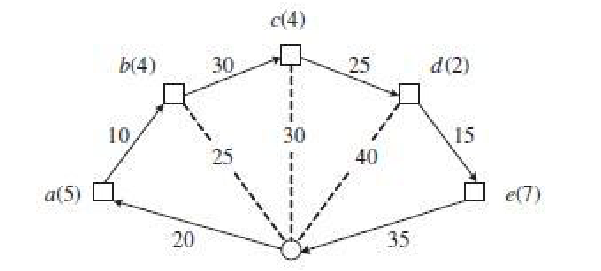
\includegraphics[width=0.6\columnwidth]{img/VRP2}
\end{center}
the arcs corresponding to unfeasible paths (weight $> W$) do not exist, the costs of the arcs are the costs of the TSP solutions for $\{d, v_{i+1}, \, ... \, , v_j \}$
\begin{center}
	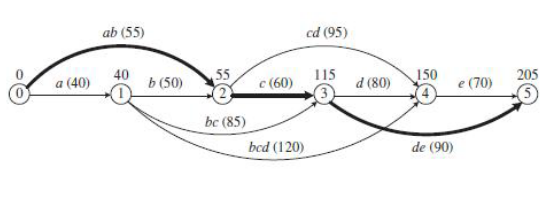
\includegraphics[width=0.6\columnwidth]{img/VRP3}
\end{center}
The optimal path corresponds to three circuits: $(d, v1, v2, d), (d, v3, d)$ and $(d, v4, v5, d)$
\begin{center}
	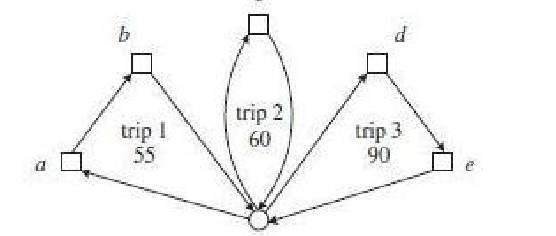
\includegraphics[width=0.6\columnwidth]{img/VRP4}
\end{center}

\newpage

\subsection{Variable Depth Search (VDS)}

In the VDS a \textbf{composite move} is a \textbf{sequence of elementary moves}
\begin{itemize}
	\item Consider each solution $x'$ in the basic neighborhood $N_{\mathcal{O}_1} (x)$.\\
	
	\item From it, make a sequence of moves \textbf{optimizing each elementary step}, but \textbf{allowing worsening moves} and \textbf{forbidding backward moves}.\\
	
	\item \textbf{Terminate} when the \textbf{current solution} $y$ becomes \textbf{worse than} $x'$ or \textbf{all moves are forbidden} (the length $k$ of the sequence is variable).\\
	
	\item \textbf{Return} the \textbf{best solution} $y^\ast$ \textbf{found} along the sequence.\\
\end{itemize}

\paragraph{Scheme of the VDS:} Given $x^{(t)}$, for each $x' \in N (x^{(t)})$, instead of evaluating only $f (x')$
\begin{enumerate}
	\item Find a promising solution $\tilde{y}$ in a neighborhood $\hat{N} (x') \subseteq N (x')$.\\
	
	\item As long as $\tilde{y}$ improves $x^{(t)}$, replace $x'$ with $\tilde{y}$ and go to $1$.\\
	
	\item Return the best solution $y^\ast$ found during the whole process.\\
\end{enumerate}

\newpage

\begin{center}
	For each $x' \in N (x)$
\end{center}

\begin{algorithm}
	\caption{Steepest Descent}
	\begin{algorithmic}
		\STATE Compute $f(x')$
	\end{algorithmic}
\end{algorithm}

\begin{algorithm}
	\caption{Variable Depth Search}
	\begin{algorithmic}
		\STATE $y := x'$; $y^\ast := x'$; Stop $:= false$;
		\WHILE{Stop $=false$}
		\STATE $\tilde{y} := \arg \min_{y' \in \hat{N}(y)} f(y')$
		\IF{$f (\tilde{y} ) \geq f (x')$}
		\STATE Stop $:= true$
		\ELSE
		\STATE $y := \tilde{y}$
		\ENDIF
		\IF{$f (\tilde{y} ) < f (y^\ast)$}
		\STATE $y^\ast := \tilde{y}$
		\ENDIF
		\ENDWHILE
		\RETURN $f (y^\ast)$;
	\end{algorithmic}
\end{algorithm}
It is a sort of roll-out mechanism for exchange algorithms.\\

Instead of just computing the value of the function in $x'$, you try to "launch" a local search heuristic; starting from $x'$ you repeatedly explore a neighborhood of the current solution $\tilde{y}$, as long as you don't satisfy a termination condition, keeping track of the best solution found all along.\\

You get a candidate solution and then you explore, starting from that solution, a (much) smaller neighborhood (to have a fast exploration) and repeat this cycle until a termination condition holds, i.e. when the new solution is worse than the original one.\\

By accepting worsening moves (with a bound in the original solution) it allows to go further in the search space than a simple steepest descent.\\

\newpage

\paragraph{Differences to steepest descent:} With respect to steepest descent exploration
\begin{itemize}
	\item VDS \textbf{finds a local optimum for each solution of the neighborhood} performing a sort of one-step look-ahead.\\
	
	\item VDS \textbf{admits worsenings along the sequence} of elementary moves (but never with respect to the starting solution).\\
	
	\item VDS \textbf{makes moves that increase the distance from the starting point} to avoid cyclic behaviors (gradually restricting the neighborhood).\\
\end{itemize}

In order to limit the computational effort
\begin{itemize}
	\item the \textbf{elementary moves} use a \textbf{reduced neighborhood} $\hat{N} \subseteq N$
	
	\item $\hat{N}$ (elementary step) is \textbf{explored} with the \textbf{first-best strategy} (as soon as you find an improvement you take it)
	
	\item $N$ (basic neighborhood) is \textbf{explored} with the \textbf{first-best strategy}
\end{itemize}

Instead of just computing the objective function you're trying to "have a look" far away.\\

\newpage

\subsubsection{Lin-Kernighan's algorithm for the symmetric TSP}
Still the best performing algorithm for the TSP (a variation of it).\\

Neighborhood $N_{\mathcal{R}_k} (x)$ includes the solutions obtained
\begin{itemize}
	\item deleting $k$ arcs of $x$
	
	\item adding other $k$ arcs that recreate a Hamiltonian circuit
	
	\item possibly inverting parts of the circuit (leaving the cost unchanged)
\end{itemize}

Lin-Kernighan's algorithm is a VDS with \textbf{sequences of 2-opt exchanges}: a $k$-opt exchange is equivalent to a sequence of $(k - 1)$ 2-opt exchanges, where each deletes one of the two arcs added by the previous exchange.\\

Then for each solution $x' \in N_{\mathcal{R}_2} (x)$ obtained by exchange $(i, j)$
\begin{itemize}
	\item evaluate the 2-opt exchanges that delete the added arc $(s_i , s_{j+1})$ and each arc of $x \cap x'$ to find the best exchange $(i', j')$
	
	\item if this improves upon $x$, perform exchange $(i', j')$, obtaining $x''$
	
	\item evaluate the exchanges that delete $(s_{i'}, s_{j'+1})$ and each arc of $x \cap x''$ ...
	
	\item ...
	
	\item if the best solution among $x', x'', \, ...$ is better than $x$, accept it
\end{itemize}

It essentially does a 2-opt exchange among 2 arcs and then deletes one (fixed) and takes time $O(n)$ to search the best possible exchange across all other nodes in the solution. Reverse the path among nodes when needed. Example not provided, too long (L14 slides).\\

The arc to be removed is never the one chosen after the search, always the other one, it would be a backward move otherwise.\\

\newpage

\paragraph{Implementation details:}
\begin{itemize}
	\item \textbf{Each step deletes an arc of the starting solution} to avoid going back and one of the arcs added in the previous step to reduce complexity.\\
	
	\item This imposes an \textbf{upper bound on the length of the sequence}.\\
	
	\item \textbf{Stopping the sequence as soon as the solution is no longer better than the starting solution does not impair the result}
	\begin{itemize}
		\item the total variation of the objective sums the effect of the single moves
		$$ \delta f_{o_1, \, ... \, , o_k} (x) = \sum_{\ell = 1}^k \delta f_{o_{\ell}} (x) $$
		
		\item every sequence of numbers with negative sum admits a cyclic permutation whose partial sums are all negative
		
		\item therefore, there is a cyclic permutation of the moves $o_1, \, ... \, , o_k$ that is, improving at each step (these last two points have already been discussed)
	\end{itemize}
\end{itemize}

\newpage

\subsection{Iterated greedy methods (destroy-and-repair)}

Every \textbf{exchange} can be seen as a \textbf{combination of addition and deletion}
$$ x' = x \cup A \setminus D $$
with $A = x' \setminus x$ and $D = x \setminus x'$.\\

However
\begin{itemize}
	\item single swaps $x' = x \cup \{j\} \setminus \{i\}$ \textbf{can give bad or unfeasible results}
	
	\item \textbf{larger neighborhoods} can be \textbf{inefficient}
	
	\item in many problems \textbf{the right cardinalities of} $A$ \textbf{and} $D$ \textbf{are unknown}, because the solutions have nonuniform cardinality (e.g., KP, SCP. . . )
\end{itemize}

A possible idea is to
\begin{enumerate}
	\item \textbf{delete from} $x$ a \textbf{subset} $D \subset x$ of \textbf{cardinality} $\leq k$ (destroy heuristic)
	\item \textbf{complete it with a constructive heuristic} (repair heuristic)
\end{enumerate}

\textbf{or}, of course, \textbf{the opposite}
\begin{enumerate}
	\item add to $x$ a set $A \subset B \setminus x$ of cardinality $\leq k$
	\item reduce it with a destructive heuristic
\end{enumerate}

\paragraph{Selection of $A$ and $D$:} Most of the time both subsets are chosen heuristically, not exhaustively
\begin{itemize}
	\item tuning their size $|A|$ and $|D|$ with some parameter
	
	\item selecting promising elements based on their cost/value
	
	\item applying the first-best strategy (immediately accept any improving solution)
\end{itemize}

Usually both subsets are chosen in a randomized way (metaheuristics then). \\

% End of L15, L16 is lab, L17 ahead

\newpage